\chapter{Conformal QFT and scale invariance}
Conformal symmetry is, loosely speaking, invariance under rescaling. Conformally invariant
systems possess no intrinsic length, mass or energy scale. In particular there exists no notion of
massive particles or massive excitations as these would induce a reference scale.
Conformal invariance plays an important role in many physical systems such as
\begin{enumerate} 
\item  string theory, where the worldsheet theory is a two-dimensional conformal field theory;
\item at fixed points of the renormalisation group (RG) equations in QFT, at which a theory
becomes scale invariant;
\item  near critical points in condensed matter or statistical physics, at which the correlation
length diverges, leaving us again with a scale invariant theory;
\item the AdS/CFT correspondence, which relates gravity on AdS space with a CFT on its
boundary.
\end{enumerate}
The treatment of such conformally invariant theories necessarily differs from the treatment of
non-conformal systems in usual QFT. Two-dimensional conformal field theories are even more
special because in two dimensions the group of infinitesimal conformal transformations is infinite.
This is large enough as to sometimes allow us to solve the theory exactly and completely. Such
theories are called \emph{integrable} and the search for integrable structures also in higher dimensional
theories, e.g. for certain field theories in four dimensions (N =4 Super-Yang-Mills theory), has
become an important challenge in theoretical physics. The treatment of two-dimensional CFTs
makes use of powerful methods of holomorphic analysis and has developed into an independent
field of mathematical physics.
\section{Introduction}
CFT is a QFT with no notion of scale. CFTs have an additional global spacetime symmetry additional to Poincaré symmetry. This additional symmetry destroy, by the Coleman Mandula theorem, the mass gap in the Källen Lehman spectral densityof the propagator. In fact, in interacting CFTs interactions do not die off with time, so there i no way to define in- and out states and therefore the S-matrix does \emph{not} even exist.\\
CFTs in $\md=4$ are encountered in QFTs near fixed points of $\beta$-functions, where by definition
\begin{equation*}
	\beta(g(\mu^*)) = 0,
\end{equation*}
such that the theory is \emph{approximately} scale invariant (which in many cases implies conformal invariance) in the vicinity of the energy scale $\mu^*$. An example is asymptotically free QCD with $\mu^*=\infty$. There exist QFTs that are exact CFTs at any energy scale, but they are usually free theories in $\md=2$.\\
The non-interacting nature makes these theories uninteresting from the QFT perspective. However, they appear in an interesting way in string theory, where the fields are functions not of spacetime, but live on the $2$ dimensional surface of the trajectory of a string. The string theoretic interpretation of these $\md=2$ CFTs then gives rise to a remarkable amount of complexity, including all of QFT as a limiting case.




\section{Conformal transformations}

\begin{mybox}{Conformal transformation}
	A \emph{conformal transformation} (CT) is a diffeomorphism under which the metric scales by an overall spacetime dependent positive factor,
i.e. for $\mR^{m,n}$ with $m+n=\md$ a conformal transformations is then a diffeomorpshim $x\rightarrow x^\prime(x)$ such that
	\begin{equation}
	\label{eq:ctFull}
		x \rightarrow x^\prime \text{ such that } \frac{\partial x^\alpha}{\partial x^{\prime \mu}} \frac{\partial x^\beta}{\partial x^{\prime \nu}} \eta_{\alpha \beta} = e^{\omega(x)} \eta\munu 
	\end{equation}
	for some \emph{conformal factor} $e^{\omega(x)}$.  For infinitesimal transformations
	\begin{equation}
	\label{eq:ctInfinitesimal}
		x^{\prime \mu} = x^\mu - \epsilon^\mu (x) + \mO(\epsilon^2), \quad e^{\omega(x)} = 1 + \omega(x) + \mO(\omega^2).
	\end{equation}
	Conformal transformations obey the \emph{conformal Killing equation}
	\begin{equation}
		\label{eq:ctKilling}
		\partial_\mu \epsilon_\nu + \partial_\nu \epsilon_\mu = \omega(x) \eta\munu.
	\end{equation}
	This is a generalized form of the Killing equation, which is obtained by setting the scaling factor to $1$, i.e. $\omega=0$.
\end{mybox}
Some useful and instructive identities in $\md$ spatial dimensions are
\begin{align}
	\label{eq:ctConstraints}
	2 (\partial \cdot \epsilon) & = \md \omega(x) \nonumber \\
	(\md-1)\partial^2 \omega &= 0 \nonumber \\
	\left[\eta\munu \partial^2+(\md-2) \partial_\mu \partial_\nu \right] \omega(x) &= 0.
\end{align}
Technically, this is the origin why we must distinguish the cases $\md=2$ and $\md\geq 3$: \\
For $\md=2$ the third equation is vacuous.
\subsection{Comment on GR }
Note that for theories including gravity, diffeomorphism invariance is already in place. Equation \ref{eq:ctKilling} can be read as an infiniteismal diffeomorphism
\begin{align}
	\delta X^\mu &= \epsilon^\nu \partial_\nu X^\mu = \epsilon^\mu \\
	\delta g\munu &= \partial_\mu \epsilon_\nu + \partial_\nu \epsilon_\mu
\end{align}
cancelling the contribution from a Weyl transformation
\begin{align}
	\delta X^\mu &=0 \\
	\delta g\munu &= \omega(x) g\munu 
\end{align}
such that 
\begin{equation*}
	\delta g\munu = \delta g\munu(\text{Diff}) + \delta g\munu(\text{Weyl}),
\end{equation*}
but there is still a local rescaling since $\delta X^\mu \neq 0$.

\subsection{On symmetry}
A conformal field theory (CFT) is a field theory that is invariant under \emph{infinitesimal} conformal transformations. In a theory of gravity (i.e. a diffeomorphism invariant theory), conformal invariance is a gauge symmetry. In a fixed background theory, conformal invariance is a global symmetry implying conserved currents.







\section{Classification of conformal transformations}
\subsection[The conformal group in greater or equal to three dimensions]{The conformal group in $\md$ $\geq 3$}
The set of \emph{infinitesimal} conformal transformations can be deduced by finding the most general solution of the constraints \ref{eq:ctConstraints}.
\begin{mybox}{Infinitesimal conformal transformations}
Infinitesimal conformal transformations make up the conformal symmetry group, consisting of the Poincaré group, dilations and special conformal transformations
\begin{align}
	&X^\mu \rightarrow X^\mu + a^\mu \quad \text{translations} \\
	&X^\mu \rightarrow X^\mu + m^\mu_\nu x^\nu \text{ with }m\munu=-m_{\nu \mu} \quad \text{Lorentz trafos}\\
	&X^\mu \rightarrow (1+\alpha) X^\mu \quad \text{dilatations} \\
	&X^\mu \rightarrow X^{\prime \mu}= X^\mu + 2 (X\cdot b) X^\mu - (X\cdot X) b^\mu \quad \text{special CTs } 
\end{align}
with infinitesimal parameters $a,m, \alpha,b$.
\end{mybox}
\subsubsection{The special conformal transformations (SCT)}
The \emph{global version} of the special conformal transformations is
\begin{equation}
	\frac{x^\prime}{(x^\prime \cdot x^\prime)} = \frac{x}{(x \cdot x)} - b.
\end{equation}
This can be understood as a successive application of an inversion $x\rightarrow \frac{x}{x^2}$, a translation and another inversion .\\
Note that (finite) global special conformal transformations take the form
\begin{equation}
	X^\mu \rightarrow \frac{X^\mu - (X\cdot X) b^\mu}{1-2(b\cdot X) + (b\cdot b) (X\cdot X)}.
\end{equation}
This is infinite at those points where the denominator vanishes. We conclude that in order for special conformal transformations to be globally defined we must consider the \emph{conformal compactification} $\mR^{n,m}\cup \infty$. \\
This shows that we must carefully distinguish between
\begin{enumerate}
	\item The group of \emph{globally defined} conformal diffeomorphisms, called \emph{conformal group} and its algebra, the \emph{conformal algebra} and
	\item the group of \emph{infinitesimal} conformal transformations.
\end{enumerate}
In particular, the conformal group depends on the topology of the space we consider as seen above. E.g. for $\mR^{n,m} \cup \infty$ and $\md =n+m \geq 3$ the conformal group has $\half (\md+1)(\md+2)$ parameters. indeed one can prove the following theorem
\begin{mybox}{}
The conformal group acting on $\mR^{n,m} \cup \infty$ is isomorphic to $SO(m+1,n+1)$.
\end{mybox}

\section{Conformal transformations of (classical fields)}
We want to find out in which representation fields transform under a transformation of the conformal group.
\subsubsection{Local fields}
The fundamental objects in a CFT are \emph{local} fields, where local means that $\phi=\phi(x^\mu)$, $x^\mu \in \mR^{1,3}$.\footnote{These become local operator under quantization.} Knowing all the operators (i.e. knowing their rep., i.e. their dimension) and their correlation functions amounts to solving the complete theory (for a CFT).\\
In a theory with a Lagrangian, the fields will simply be linear combinations of products of (derivatives) the \emph{fundamental fields}. Consider a scalar field theory as an example. Here the fundamental field is $\phi(x)$. The fields, in a CFT sense, then are the possible linear combinations
\bse
\mO_1(x)=\phi(x),\;  \mO_2(x)=\phi^n(x),\; \mO_{3,\mu} (x) = \partial_\mu \phi(x),\; \mO_{4,\mu}(x)=\phi(x) \partial_\mu \phi(x), \; \dots 
\ese 
In a gauge theory, we must ensure that the fields are gauge-invariant, i.e. looking for invariant combinations of the fundamental field $A^\mu$, which in of itself is not gauge-invariant.
\\
\\
In the following, we will consider the respective contributions to the conformal group separately.
\subsubsection{Transformation behaviour of fields under the Lorentz group}
Compare \ref{subsec:lorentzrep}.

\subsubsection{Transformation behaviour of fields under Dilatations}
One defines the \emph{dilatation weight} 
\be
\label{eq:cftdilatationweight}
\Delta = + [\mO], \qquad \text{for any local operator } \mO.
\ee 
If you have a length scale and expand or shrink it, e.g. if you perform the following dilatation on a scalar field
\bse
x^\mu \rightarrow \lambda x^\mu,\qquad [\phi] = \frac{\md-2}{2},
\ese 
then we have
\bse 
\phi \stackrel{x\rightarrow \lambda x}{\longrightarrow} \phi^\prime (x^\prime) = \lambda^{- [\phi]} \phi(x).
\ese 
\begin{mybox}{Dilatation}
	More generally, \emph{all} local operators have a dilatation weight $\Delta$ such that they transform under a dilatation $x\rightarrow \lambda x$ like
	\begin{equation}
		\mO \longrightarrow \mO^\prime(x^\prime) = \lambda^{-\Delta} \mO(x),\quad \Delta = [\mO].
	\end{equation}
\end{mybox}

\subsubsection{Primary fields - useful for general conformal transformations}
When considering more general conformal transformations, we first have to consider so-called \emph{primary fields}.
\begin{mybox}{Primary field}
	A scalar primary field $\mO(x)$ with weight $\Delta$ transforms under a general conformal transformation as
	\begin{equation}
	\label{eq:cftPrimaryfields}
	\mO \longrightarrow \mO^\prime (x^\prime) = \Omega(x)^{-\Delta} \mO(x),
	\end{equation}
	where we have infinitesimally
	\begin{equation}
		\label{eq:cftPrimaryfieldsInfinitesimal}
		\delta \mO(x) = - \kappa(x) \Delta \mO(x) - \xi^\mu \partial_\mu \mO(x).
	\end{equation}
	\emph{Descendents} is the name for derivatives of primaries.
\end{mybox}
A non-scalar primary field has a dilatation weight $\Delta$ and transforms in a representation of the Lorentz group $SO(1,D-1)$. indicate the Lorentz rep. by an index $I \in \{\alpha,\dot{\alpha},\mu,\dots \}$. It transforms under an infinitesimal conformal transformation
\begin{equation}
	\delta\mO_{\Delta, I} (x) =- \kappa(x) \Delta \mO_{\Delta,I} (x) -\xi^\mu (x) \partial_\mu \mO_I(x) +\rho^\mu_\nu(x) \left(S^\nu_\mu\right)^J_I \mO_J(x) 
\end{equation}
with $S$ being the representation matrix in question for the Lorentz trafo (i.e. for spinors \ref{eq:spinortrafo}) and
\begin{align*}
\kappa(x) &= \sigma - 2 b \cdot x \\ 
\rho^\mu_\nu(x) &= \omega^\mu_\nu + 2 \left(b^\mu x_\nu - x^\mu b_\nu \right),\\
\xi^\mu(x) &= a^\mu + \omega^\mu_\nu x^\nu + \sigma x^\mu + b^\mu x^2 -2 x^\mu b\cdot x.
\end{align*}
\begin{mybox}{Transformation behaviour of primary fields}
By taking coefficients of $b, a_\mu,  \sigma, \omega^{\mu \nu}$, we get te action of $P_\mu, K_\mu, D,J_{\mu \nu}$
\begin{align}
	\label{eq:cftPrimaryTrafo}
\delta_D &= - (\Delta +x^\mu \partial_\mu),\\
\delta_{K_\mu} &= 2 x_\mu \Delta - (x^2 \partial_\mu - 2 x_\mu x^\nu \partial_\nu) + 4(x_\nu S^\nu_\mu)\nonumber,\\
\delta_{P_\mu} &= -\partial_\mu \nonumber, \\
\delta_{J_{\mu \nu}} &= \nonumber.
\end{align}
\end{mybox}
Note that not all local fields are primary, but all local fields can be written as a linear combination of primary fields and descendents of primaries via the OPE \ref{eq:cftOPE}.
\subsection{Examples of fields}
Consider a free, massless, complex scalar field theory. This is a CFT
\bse 
S =\int \md^d x \partial_\mu \phi \partial^\mu \phi^\dagger, \qquad [\phi]=\frac{\md -2}{2},
\ese 
where $\phi,\phi^\dagger$ is a scalar primary operator. We can now built operators and test whether they are primary or descendant. Consider for example
$\phi \partial_\mu \phi^{\dagger}$, we find that
\bse 
\partial_\mu(\phi \phi^\dagger) = \phi \partial_\mu \phi^\dagger + (\partial_\mu \phi) \phi^\dagger 
\ese 
is a descendent, but that
\bse 
\phi \partial_\mu \phi^\dagger -\phi^\dagger \partial_\mu \phi 
\ese 
is a primary with dilatation weight
\bse 
\Delta = \frac{\md-2}{2} + 1+\frac{\md-2}{2} = \md -1.
\ese 
This can be seen that by checking that this object has the correct $\delta_{K_\mu},\delta_D$ for a primary field.


\subsection{Energy-Momentum tensor as a primary field in CFT,}

$T^{\mu \nu}$ is a field in \emph{every} CFT. Simplest way to define it is\footnote{assuming there to exist a Lagrangian for the theory, otherwise it is just an operator transforming with dilatation weight and in a specific rep under Lorentz trafo} is by coupling the theory to gravity as seen in my GR note \todo{Maybe Merge at some point ?}
\bse 
S = \int \md^4 x \partial_\mu \phi \partial^\mu \phi \longrightarrow \int \md^4 x \sqrt{-g} \nabla_\mu \phi \nabla_\nu \phi g^{\mu \nu}.
\ese 
The usual definition of energy momentum tensor ensuring translation invariance on a fixed background
\begin{equation}
\delta S =: \int \md^d x \sqrt{-g} T^{\mu \nu} \delta g\munu \; \Leftrightarrow \; T^{\mu \nu} = \frac{1}{\sqrt{-g}} \frac{\delta S}{\delta g\munu }.
\end{equation}

\subsubsection{Properties of the Energy-Momentum tensor}
\begin{enumerate}
	\item \begin{mybox}{Weyl invariance of the energy momentum tensor}
		In CFT, we have invariance under $g\munu\rightarrow e^\lambda g\munu$ where
		\begin{equation}
		\delta g\munu = \lambda g\munu,
		\end{equation}
		this implies
		\begin{equation}
		0= \delta S = \int \md^d x \frac{\delta S}{\delta g\munu}\delta g\munu = \int \md^d x \sqrt{-g} T^\mu_\mu, \; \Leftrightarrow T^\mu_\mu =0,
		\end{equation}
		i.e. the energy momentum tensor of conformal field theories is \emph{traceless}.
	\end{mybox}\footnote{Remark: Can have \emph{Weyl anomaly} in every $\md =2n$ CFT, which effects the infinitesimal trafo.}
\item Since this theory is coupled to gravity, it is diffomorphism invariant, i.e.
\be 
\label{eq:cftDiffeomorphismInvariance}
\delta S=0 \text{ under } \delta g\munu= \partial_{(\mu} \xi_{\nu)}.
\ee 
This implies the conservation equation
\be 
\partial_\mu T^{\mu \nu} = 0.
\ee 
Note that energy-momentum conservation holds here because we are considering Minkowski, i.e. flat space.
\item 
\begin{mybox}{}
	In any CFT
	\begin{equation}
	T^{\mu \nu} \text{ is a primary of scaling dimension $\md$ and conformal spin }2.
	\end{equation}
\end{mybox}
\end{enumerate}
\subsubsection{Noether currents }
From $T^{\mu \nu}$ we can construct \emph{all} the Noether currents associated with conformal symmetries.
\bse 
 \begin{tabular}{lll}
	matter field          & current & conserved \\
	\toprule
	\text{Translations, }$ \partial_\mu$ & $T^{\mu \nu}$ & $P^\mu = \int T^{\mu 0} \md^3x$ \\
	\text{Any conformal trafo } $\xi^\mu \partial_\mu$ & $j^\mu = T^{\mu \nu} \xi_\nu$ & $Q_S = \int T^{0 \nu} \xi_\nu \md^3x$\\
	\bottomrule
\end{tabular}
\ese 
Conservation of the Noether current then stems from the conformal Killing equation \ref{eq:cftKilling}
\begin{align*}
	\partial_\mu j^\mu &= \underbrace{\partial_\mu T^{\mu \nu}}_{=0} \xi_\nu + T^{\mu \nu} \partial_\mu \xi_\nu \stackrel{T^{\mu \nu} = T^{\mu \nu} }{=} T^{\mu \nu} \partial_{(\mu} \xi_{\nu)} \\
	&\stackrel{\ref{eq:cftKilling}}{=} k \eta\munu T^{\mu \nu} = k \underbrace{T^\mu_\mu}_{=0} = 0
\end{align*}
and from the tracelesness of the energy-momentum tensor. For example, the current of dilatations $\xi^\nu = \sigma x^\nu$ is $T^{\mu \nu} x_\nu$. This is a general statement. For symmetries being represented by Killing vectors $\{ \xi_\mu \}$ one has conserved currents 
\be 
\{ j^\mu = T^{\mu \nu} \xi_\nu				\}.
\ee 



\section{Correlation functions, the heart of CFT}
\subsection{Foreword}

A CFT is a physical theory invariant under the group of \emph{infinitesimal} conformal transformations.
In particular, as anticipated already, there is no intrinsic notion of length scale or of massive excitations.\\
\\
Even though the definition of a CFT is much more general, let us first take the Lagrangian
perspective, whose logic is familiar from the definition of general QFTs:
\begin{enumerate} 
	\item  Our starting point is a classical theory defined by an action $S[\phi_i(x)]$ with the specific
	requirement that this action is invariant under infinitesimal conformal transformations.
	\item  The basic objects of this theory are the \emph{fields} $\mO_i(x)$. By this we mean, by slight abuse of
	notation, any \emph{local expression} built out of the $\phi_i(x)$  appearing in the action and derivatives
	thereof. Local fields are e.g. products or power series such as exponentials of $\phi_i(x)$. These $\mO_i(x)$ are also called \emph{ local operators}.
	\item  The quantum theory is determined by the correlation functions
	\begin{equation}
	\langle \mO_1(x_1) \dots \mO_n(x_n) \rangle = \frac{1}{Z} \int \md \phi_i e^{- S[\phi_i]} \mO_1(x_1) \dots \mO_n(x_n).
	\end{equation}
	Importantly, the expression inside $\langle \dots \rangle$ is always time-ordered as is familiar from the treatment of correlation functions in usual QFTs.
	\item  In writing equations involving the local $\mO_i$ we will always think of operator equations in
	the full quantum theory, i.e. think of the operators as inserted into a time-ordered path
	integral as above. For instance an equation of the form
	\begin{equation}
	\mO_1(x_1) \mO_2(x_2) = f(\mO_1(x_1),\mO_2(x_2)) 
	\end{equation}
	is shorthand for
	\begin{equation}
	\label{eq:ct1}
	\langle \mO_1(x_1) \mO_2(x_2) \dots \rangle = \langle f(\mO_1(x_1),\mO_2(x_2))\dots \rangle
	\end{equation}
	with $\dots$. representing arbitrary operator insertions at a distance bigger that $\abs{x_1-x_2}$.
	
\end{enumerate}

Now comes an important, though probably unfamiliar point: Conformal symmetry allows for a
rather different definition of the theory than the one above starting from a classical action. A
generic CFT in $\md$ dimensions need not have a description via an action. Rather it is defined
by a ’complete set’ of local fields $\mO_i$ and their correlation functions. If we do have a Lagrangian
description, these correlation functions are given as above. More generally, however, we can think
of the correlators as maps from the space of operators to $\mathbb{C}$ consistent with conformal invariance.
We will see that this is very constraining. If really all correlators are known in terms of a finite
amount of input data the theory is solved completely and defined through these data.\footnote{A CFT in $\md = 2$ dimensions is indeed exactly solvable in this sense. This is because the two-dimensional
	Virasoro algebra is infinite-dimensional. In higher dimensional CFTs the computation of all correlators in terms
	of finite data is possible in principle, but much harder in practice due to the lack of this extra symmetry.}
There are essentially two reasons why this can work: First, because there is a special notion of
a ’complete set of operators’ available in a CFT which does not exist in a general QFT - the set
of quasi-primary fields - and second, because the operator product expansion (OPE) of two such
quasi-primaries has remarkable properties. Let us introduce both concepts in turn.
\subsection{Primary and quasi-primary fields}
As most people are interested in the applications of two-dimensional CFTs to string theory, we restrict the following discussion, unless stated otherwise, to a $\md=2$ CFT on $S^2= \mathbb{C}\cup \infty$, with general fields of the form $\mO(z,\bar{ z})$.
\begin{enumerate}
	\item If a field $\Phi(z,\bar{ z})$ transforms under $z\rightarrow z^\prime =\lambda z$, $\lambda \in \mathbb{C}$ as
	\begin{equation}
	\Phi(z,\bar{ z}) \rightarrow \Phi^\prime (z^\prime ,\bar{ z}^\prime) = \lambda^{-h} \bar{\lambda}^{-h\bar{h}} \Phi(z,\bar{z})
	\end{equation}
	then it has \emph{conformal dimension} $(h,\bar{h})$. Note that in general $\bar{h} \neq h^*$.
	\item A \emph{primary field} $\Phi(z,\bar{z})$ transforms as a tensor under conformal transformations $z\rightarrow z^\prime = f(z)$:
	\begin{equation}
	\label{eq:ctPrimaryfield}
	\Phi(z,\bar{z}) \rightarrow \Phi^\prime(z^\prime,\bar{z}^\prime) = \left(\frac{\partial f}{\partial z}\right)^{-h} \left(\frac{\partial \bar{f}}{\partial \bar{z}}\right)^{-\bar{h}} \Phi(z,\bar{z}).
	\end{equation}
	Note that in particular, and in the spirit of the discussion around \ref{eq:ct1}, we require as part of the defining property of a primary field that any correlation function involving primary fields transforms as
	\begin{equation}
	\langle\prod_i \Phi(z_i,\bar{z}_i)\rangle \rightarrow \prod_i \left(\frac{\partial f}{\partial z}|_{z_i}\right)^{-h_i} \left(\frac{\partial \bar{f}}{\partial \bar{z}}|_{\bar{z}_i}\right)^{-\bar{h}_i} \langle \prod_i \Phi(z_i,\bar{z}_i)\rangle.
	\end{equation}
	Expanding $f(z) = z + \epsilon(z)+\dots$ gives the infinitesimal scaling behaviour for primary fields
	\begin{equation}
	\delta_{\epsilon,\bar{\epsilon}} \Phi(z,\bar{z}) = -\left(h \partial_z \epsilon + \epsilon \partial_z +\bar{h} \partial_{\bar{z}} \bar{ \epsilon} + \bar{ \epsilon} \partial_{\bar{z}}\right) \Phi(z,\bar{ z}).
	\end{equation}
	\item A \emph{quasi-primary field} satisfies \ref{eq:ctPrimaryfield} for $f\in PSL(2,\mathbb{C}) = SL(2,\mathbb{C}) /\mathbb{Z}_2$. In particular, every primary is a quasi-primary, but not the other way round.
	
	\item A \emph{chiral field} is a field $\Phi(z)$, an anti-chiral field is a field $\Phi(\bar{ z})$.
\end{enumerate}
Remarks:
\begin{enumerate}
	\item	Quasi-primaries are tensors under the group of globally defined conformal transformations.
	In a $\md$-dimensional CFT with $\md > 2$ (on $\mR^{ m,n}$ with $m + n = \md$), these are the fields with
	specific transformation behaviour under $SO(m + 1, n + 2)$. \footnote{Note
		that in many texts on higher-dimensional CFTs the term primary is used for what we call quasi-primary.} All the statements we make
	about the quasi-primaries based on their transformations under $PSL(2, \mathbb{C})$ transformations
	in a two-dimensional CFT carry over analogously to quasi-primaries in higher-dimensional
	CFTs.
	\item What has no analogue in higher dimensions is the concept of a primary field, which exploits
	the infinitesimal structure of the two-dimensional Virasoro algebra.
\end{enumerate}

\subsection{The quantum theory, a first idea}
Now we consider the quantum theory. Local fields get promoted to local operators acting on some Hilbert space. Conformal transformations act as in the classical case
 expect that now the symmetry can be implemented via operators as a commutator term. Therefore we have that the generators of the conformal group $D, K_\mu, P_\mu, J_{\mu \nu}$ becoming operators defined via $T^{\mu \nu}$ as above to have
\begin{mybox}{Defining commutators of the conformal algebra}
	\begin{align}
	[D,\mO(x)] &= - \delta_D \mO \\
	[K_\mu, \mO(x) ] &= - \delta_{K_\mu} \mO \\
	[P_\mu, \mO(x)] &=-\delta_{P_\mu} \mO \\
	[J\munu, \mO(x)] &= - \delta_{J\munu} \mO.
	\end{align}
\end{mybox}
The key objects in CFT are local operators and the key \emph{data} defining the CFT are \textbf{the correlation functions of these local operators}. Thus, the key objects are vacuum expectation values
\begin{mybox}{} 
	\be 
\expval{\mO(x_1) \dots \mO(x_n)} = \expval{\mO(x_1) \dots \mO(x_n)}{0} = f(x_1,\dots,x_n).
\ee

\end{mybox}
If we know all the correlators, we say that we have solved the theory, because we can compute anything of the theory from the correlation functions. We will see later on, that the OPE \ref{eq:cftOPE} allows us to reduce every expression of interest down to three-point functions.\\
This is way easier than computing everything via Feynman diagrams, as we get a lot of info on the theory already from the conformal symmetry. What conformal symmetry tells us about these correlation functions is explained in the following.

\subsection{Conformal symmetry of correlation functions}
\begin{mybox}{Ward identity CFT}
If $x\rightarrow x^\prime$ is a quantum symmetry (symmetry of QFT, i.e. $S=S^\prime$) with $\mO\rightarrow \mO^\prime$ for primary operators $\{\mO_i\}$ with respective weights $\{\Delta_i\}$, then
\bse 
\expval{\mO(x_1) \dots \mO(x_n)} = \expval{\mO^\prime(x_1) \dots \mO^\prime(x_n)},
\ese 
which is infinitesimally
\begin{align}
	\label{eq:cftWard}
	\expval{\delta \mO_1(x_1) \mO_2(x_2) \dots \mO_n(x_n) } & \expval{\mO_1(x_1) \delta\mO_2(x_2) \dots \mO_n(x_n) } \\
	&+ \expval{\mO_1(x_1) \dots \mO_{n-1}(x_{n-1}) \delta \mO_n(x_n)} = 0 \nonumber.
\end{align}
For a CFT, conformal transformations are quantum symmetries, such that \ref{eq:cftWard} is true for all infinitesimal conformal transformations.
\end{mybox}
\begin{enumerate}
	\item For translations with $\delta= \delta_{P_\mu} =- \partial_\mu$ this gives
\be 
\label{eq:cftWardTranslation}
\left(\frac{\partial}{\partial x^\mu_1} + \dots + \frac{\partial}{\partial x^\mu_n}\right) \expval{\mO_1(x_1) \dots \mO_n(x_n) } = 0.
\ee 
\item For Dilatations with $\delta = \delta_D = - (\Delta + x\cdot \partial)$ this gives
\be 
\label{eq:cftWardDilatations}
(x_1 \cdot \partial_1 + \dots + x_n \cdot \partial_n + \Delta_1+\dots+\Delta_n) \expval{\mO_1(x_1) \dots \mO_n(x_n)} =0.
\ee 
\item When $\mO_j(x)$ is a scalar primary with dilatation weight $\Delta_j$, then for SCT with 
\bse 
\delta = \delta_{K_\mu} = 2 x_\mu \partial^2 - (x^2 \partial_\mu - 2 x_\mu x\cdot \partial),
\ese 
we have
\begin{equation}
	\label{eq:cftWardSCT}
	\left[\sum_{i=1}^{n} \left(2 x_{i \mu} \Delta_i - \underbrace{\left(x^2_i \partial_\mu - 2 x_{i \mu} x^\nu_i \partial_{i \nu}\right)}_{= K_{i\mu}} \right)\right] \expval{\mO_1(x_1) \dots \mO_n(x_n) } = 0,
\end{equation}\footnote{Note that you will get additional terms for non-scalar primaries.}
where $K_{i\mu}$ is the generato of special conformal transformations at $x_i$. 
\end{enumerate}
These are called \emph{conformal Ward identities}. Note that only SCT and dilatation identites are new, as we already have Ward identites for the Poincaré transformations in any Poincaré invariant theory, i.e. QFT.\\
\\
We can use these Ward identities to constrain the correlators now.
\subsubsection{Two-point functions of scalar operators}
Let $\expval{\mO_1(x_1)\mO_2(x_2)}=f(x_1,x_2)$ where we assume $\mO_i(x)$ scalars\footnote{For non-scalars we have to assume that they are in the same Lorentz rep.}.We have the following constraints due to symmetry of the theory.

\begin{enumerate}
	\item Impose translation symmetry
	\bse 
	(\partial_1 +\partial_2) f(x_1,x_2) = 0 \; \Rightarrow f(x^\mu_1,x^\mu_2) = f(\underbrace{(x_1-x_2)^\mu}_{\equiv x_{12}}) 
	\ese 
	such that the correlator only depends on one variable, i.e. the distance.
	\item 
	Lorentz symmetry implies that objects only depend on contracted things, i.e. on Lorentz scalars $f=f(x^2_{12})$.
	These are the constrains we usually have on our correlators due to Poincaré-invariance of every QFT. The additional constraints due to conformal symmetry come now.
	\item Dilatations imply 
	via the chain rule
	\bse 
	\frac{\partial}{\partial x^\mu_1} f(x^\mu_{12} x_{12,\mu} ) = 2 x_{12,\mu} f^\prime(x^2_{12}), \; \partial_2 f(x^2_{12}) =-2 x_{12,\mu} f^\prime(x^2_{12}) 
	\ese 
	that \ref{eq:cftWardDilatations}
		\begin{align*}  
		\left(x_1 \cdot \partial_1 + x_2 \cdot \partial_2 + \Delta_1 + \Delta_2 \right) f(x^2_{12}) &= 0 \\
		\Leftrightarrow \quad (2 x_1 \cdot x_{12} f^\prime (x^2_{12}) - 2 x_2 \cdot x_{12} f^\prime (x^2_{12})) + (\Delta_1+\Delta_2) f(x^2_{12}) &=0 \\
		\Leftrightarrow\quad 2 x^2_{12} f^\prime(x^2_{12}) +(\Delta_1 +  \Delta_2) f(x^2_{12}) &=0.
	\end{align*}
	We can solve this equation via separation of variables with $x\equiv x^2_{12}$ 
	\bse 
	\ln f = A + \frac{\Delta_1+\Delta_2}{2} \ln x \; \Rightarrow \; f = \frac{A}{x^{\frac{\Delta_1+\Delta_2}{2}}}.
	\ese 
	Thus, we find that the two-point correlator of a theory invariant under Poincaré transformations and dilatations to be
	\begin{equation}
	\label{eq:cftCorrelatorTwoPoint1}
	\expval{\mO_1(x_1) \mO_2(x_2)} = \frac{C_{12}}{\abs{x_1 - x_2}^{\Delta_1+\Delta_2} }
	\end{equation}
	with $\abs{x_1-x_2}\equiv \sqrt{x^2_{12}}$, $[C_{12}]=0$.	
	\item SCTś imply that 
\bse 
(k_{1\mu}+k_{2\mu} ) \abs{x_{12}} = - (x_{1\mu}+x_{2\mu} ) \abs{x_{12}}.
\ese 
Now we assume that $x_{1\mu} \neq x_{2\mu}$, which is the statement of \emph{up to contact terms} in the Ward identity, which are parts of the correlator for operators being evaluated at the same spacetime point. Then, using the above equation and \ref{eq:cftCorrelatorTwoPoint1}, we find that the two-point correlator is even further constrained to be
\be
\label{eq:cftCorrelatorTwoPoint}
\expval{\mO_{\Delta, I}(x_1) \mO_{\Delta,2}(x_2) } = \left\{\begin{array}{ll}
	\frac{C_{12}}{\abs{x_1 - x_2}^{2 \Delta}} & \Delta_1= \Delta_2 = \Delta \\
		0 & \text{else}\\
	\end{array}			\right\}
	\ee 
	\end{enumerate}
	Concluding this section, we find that the conformal symmetry fixes the two-point funciton up to a number $C_{12}$. Note that therefore solving a CFT is equal to \emph{defining the space of operators and their dimensions}, where the space of operators is basically the space of two-point functions.\footnote{Note that you can anomalous dimensions $\Delta=\Delta(g)$ running with the coupling. Integrability would then tell us what the anomalous dimension is.}

\subsubsection{Three-point functions of scalar operators}
We can proceed with a similar analysis of the constraints conformal symmetry puts on the three-point correlator\footnote{E.g. translation invariance leaves us with a triangle shaped dependence of the spacetime points reducing degrees of freedom to two distances.} to find that
\be 
\label{eq:cftCorrelatorThreePoint}
\expval{\mO_{\Delta, I}(x_1) \mO_{\Delta,2}(x_2) \mO_{\Delta, 3}(x_3)} = \frac{C_{123}}{\abs{x_{12}}^{\Delta_1+\Delta_2-\Delta_3} \abs{x_{23}}^{\Delta_2+\Delta_3-\Delta_1} \abs{x_{13}}^{\Delta_1+\Delta_3-\Delta_2} }.
\ee 
Again, integrability of the theory can tell us exactly what the three-point function is. $C_{123}$ is the only physical object next to the anomalous dimension. If you kno all three-point functions and anomalous dimensions, you know the whole theory.

\subsubsection{Four-point functions of scalar operators}
These are no longer fixed by conformal symmetry, we can see this from a d.o.f. argument: We have a finite number of constrains we can put on the system and so there has to exist a point where the theory is not fully constrained anymore. Assuming scalar primaries, one finds
\be 
\label{eq:cftCorrelatorFourPoint}
\expval{\mO_1(x_1) \dots \mO_4(x_4)} = f(u,v) \underbrace{ \prod_{i<j} \abs{x_{ij}}^{\frac{\Delta_1+\Delta_2+\Delta_3+\Delta_4}{3} - \Delta_i-\Delta_j }}_{\text{solves Ward id.}},
\ee 
where we have the \emph{conformal cross ratios}
\bse 
u = \frac{\abs{x_{12}} \abs{x_{34}} }{\abs{x_{13} } \abs{x_{24}} }, \quad v= \frac{\abs{x_{14}} \abs{x_{23}} }{\abs{x_{13}} \abs{x_{24}} }
\ese 
and $f$ is an arbitrary function of $u,v$. The cross ratios satisfy
\bse 
(k_{1\mu} +\dots + k_{4 \mu} ) u = 0 = (k_{1\mu} + \dots + k_{4 \mu} ) v.
\ese

\subsubsection{Higher point functions ?}
Here there are more invariant cross ratios. These can not be fixed by conformal symmetry alone, so \emph{any} function of them solves the CFT. We will get further info from crossing symmetry and the OPE \ref{eq:cftOPE} later on.








\subsection{Radial quantization and the operator-state correspondence} 
\subsubsection{Radial quantization motivation}
We normally quantize a theory on "equal time slices", compare the canonical quantization procedure \ref{eq:canonicalQFTequaltimecommutationrel}. It is however equally possible to quantize on "equal radial slices", this is called \emph{Radial Quantization}.\\ 
We can motivate this by first considering the theory on a cylinder, i.e. we have a Euclidean (in the sense of Wick-rotated) CFT on $\mR\times S^{D-1}$, and relate it to flat space afterwards. On the cylinder we have Euclidean time $\tau$ and coordinates for $S^{D-1}$ which we fednite by $\vec{n}, \vec{n}^2=1$. Thus
\bse 
\md s^2= \md \tau^2 + \md \vec{n}^2, \quad \md \vec{n}^2 = \md \vartheta^2 + \sin^2 \vartheta \md \varphi^2,
\ese 
where $\tau$ is the vertical axis (i.e. the height) of the cylinder (sticked to the surface) and $S^{D-1}$ coordinates $\md \vec{n}^2$ describe the cross sections of the cylinder at every $\tau$. Consider now a coordinate transformation
\bse 
\tau \rightarrow r = e^\tau  \; \Rightarrow \; \frac{\md r}{\md \tau} = e^\tau = r, \; r= 0 \Leftrightarrow \tau = - \infty,
\ese 
the metric becomes
\bse 
\md s^2 = \frac{\md r^2}{r^2} + \md \vec{n}^2 = \frac{1}{r^2} \underbrace{(\md r^2 + r^2\md \vec{n}^2)}_{\text{flat metric}}.
\ese 
Thus, there exists a conformal transformation 
\bse 
\text{cylinder } \mR \times S^{D-1} \stackrel{\Omega=r=\abs{x}}{\longrightarrow} \mR^D \text{ flat space} 
\ese 
such that 
\begin{figure}[h!]
	\centering
	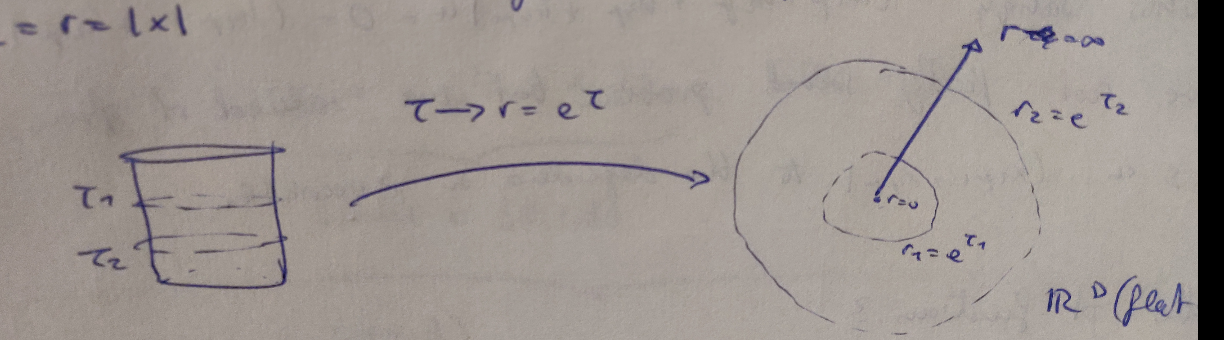
\includegraphics[width=0.63\linewidth]{gfx/Radialquantization}
	\caption{}
	\label{fig:radialquantization}
\end{figure}
Under this conformal transformation from the cylinder to flat space, we have the following $1-1$ mapping of characteristics
\bse 
 \begin{tabular}{|lll|}
 	$\mR \times S^{D-1}$ cylinder & \longrightarrow & $\mR^D$ flat space \\
	\toprule
	$\tau = -\infty$ &&$r=0$\\
	Equal time slice $\tau =\tau_1$ && Equal radius slice $r=r_1$ \\
	Ordinary (equal time) quantization && Radial quantization \\
	Special role for $\tau$ && Special rule for $r$ \\
	Time ordering && Radial ordering ($x^\mu = r n^\mu$) \\
	Time translation $\frac{\partial}{\partial t}$ && Dilatations $\frac{\partial}{\partial \ln r} = r \partial_r = x^\mu \frac{\partial}{\partial x^\mu}$ \\
	Energy of a state && Dilatation weight \\
	Scalar primary operator $\mO_{cyl}(\tau,\vec{n})$ && $\mO_{flat}(r,\vec{n}) = \mO_{cyl} (\tau,\vec{n}) \frac{1}{r^\Delta}$\\
\bottomrule 
\end{tabular}
\ese 
Comparing the hermitian conjugate on both spaces, we note that on the cylinder we have
\bse 
\mO_{cyl} (\tau,\vec{n})^\dagger = \mO_{cyl} (-\tau,\vec{n}).
\ese 
On flat space (upon radial quantization) we have 
\be 
\label{eq:cftRadialQuantizationHermitianConjugate}
\mO^\dagger_{flat}(r,\vec{n}) = \frac{1}{r^{2 \Delta}} \mO_{flat}(\frac{1}{r}, \vec{n}),
\ee 
which is equal to an inversion $I$ acting on $\mO_{flat}$. We can deduce that 
\bse 
(K^\mu)^\dagger = I K^\mu I = P^\mu
\ese 
in radial quantization.

\subsubsection{Operator-state correspondence}
\begin{mybox}{Operator-state correspondence idea}
	In CFT, there is a one-to-one correspondence between states $\ket{\psi}\in \mH$ and local operators acting on $\mH$.
\end{mybox}
\todo{Look at Tong's notes for a more in-depth discussion}

\begin{mybox}{State-operator Isomorphism}
	\begin{equation}
	\text{Local operators on the boundary }\leftrightarrow \text{ states on the interval}
	\end{equation}
	in pathintegral formalism
	\begin{equation}
	\Psi_{\mO} [\phi_b] = \int \mD \phi e^{i S[\phi]} \mO(0)|_{\phi(x)=\phi_b(x) \text{ for } x\in b}
	\end{equation}
	is Schrödinger wave functional that maps operator $\mO$ to state $\braket{\Omega}{\Psi}$.
\end{mybox}


What follows is a sketch or motivation of why that is so.\\
First consider states in QM, i.e. $1$ particle in $1$ spatial dimension. States are equivalent to solutions of the Schrödinger equation, i.e. to Schrödinger-wave functions $\psi(x,t_0)$ at time $t_0$. An initial state is obtained for
\bse 
\psi_{I} (x) = \lim_{t_0\rightarrow - \infty} \psi(x,t_0).
\ese 
We can also consider wave functions in QFT (for simplicity we consider a single scalar particle). Then
\bse 
 \begin{tabular}{|lll|}
	QM & \longrightarrow & QFT \\
	\toprule
Configuration space $x$ && $\phi(x)$ space of fields fixed at $t_0$ \\
Initial state $\psi_I(x)$ && $\lim_{t_0\rightarrow -\infty} \Psi\left[\phi(x,t_0),t_0\right]$ on spatial slices at $t_0$.\\
	\bottomrule 
\end{tabular}
\ese 
What is this functional ?
\bse 
\lim_{t_0\rightarrow -\infty} \Psi\left[\phi(x,t_0),t_0\right]\stackrel{\text{radial quant.}}{\rightarrow} \lim_{r\rightarrow0} \Psi\left[\phi(r,\vec{n}),r\right] 
\ese 
becomes a functional of $\phi(\vec{x})$ at $\vec{x}=0$ upon radial quantization. Thus, $\Psi$ is a function of $\phi(0),\partial_\mu \phi(0),$ $\partial_\mu \partial_\nu \phi(0)$, \dots, which are equivalent to the initial state as it is evaluated at $t_0\rightarrow -\infty$. This is exactly the definition of a local operator, i.e. the space of such functions at $\vec{x}=0$ is the local operator. This is because $t_0 \rightarrow -\infty$ becomes a point (i.e. local) upon radial quantization.\\
In practice, we can label our states via the corresponding operator $\ket{\mO}$ where 
\bse 
\ket{\mO}:= \mO(0) \ket{0},\quad e.g. \hat{ \mI} \leftrightarrow \ket{0}\equiv \ket{\mI}.
\ese
\marginpar{As we are looking at CFT, there is no distinction between interacting and free vacuum. This should therefore be the full vacuum}
What about a state inserting an operator at a different point, e.g. $\mO(x) \ket{0} = \ket{\psi}$ ?
\begin{align*}
\mO(x) & = \mO(0) + x^\mu \partial_\mu \mO(0) + \half x^\mu x^\nu \partial_\mu \partial_\nu \mO(0) + \dots \\
\Rightarrow \quad \ket{\psi}&= \sum_n \frac{1}{n!} x^{\mu_1} \dots x^{\mu_n} \ket{\partial_{\mu_1} \dots \partial_{\mu_n} \mO}.
\end{align*}
Note also that 
\bse
\ket{\partial_\mu \mO} =\partial_\mu \mO(0) \ket{0} = [P_\mu,\mO(0)] \ket{0}= P_\mu \mO(0) \ket{0} = P_\mu \ket{\mO}, 
\ese 
where we assumed $P_\mu \ket{0} =0$, this holds for a Poincaré invariant theory.\\
What is this good for ?\\
\begin{mybox}{}
We can think of operators as states. This means that we can label states by the dilatation weight of the corresponding operator.
\end{mybox}
To label states via the dilatation weight, we need to find out how the dilatation operator acts on states?\\
In standard QFT, we label states by their energy (amongst other quantum numbers, e.g. \ref{eq:fockstates}). Here, upon radial quantization we have seen that energy becomes the dilatation weight\footnote{this comes about a dilatation on the cylinder is a translation in time, as it is radial scaling flat space, and time translation invariance is connected to energy conservation.}\\
Consider a state $\ket{\mO_\Delta}$ where $\mO_\Delta$ is an operator (primary or descendant) with weight $\Delta$, then
\be 
\label{eq:cftStatesLabelling}
\hat{D} \ket{\mO_\Delta} =\left[[\hat{ D}, \hat{ \mO}_\Delta(0)]+\hat{\mO}_\Delta(0) \hat{D} \right]\ket{0} = \Delta \hat{\mO}_\Delta(0) \ket{0} = \Delta \ket{\mO_\Delta},
\ee 
where we used that $\hat{D} \ket{0} =0$ and that
\bse 
[\hat{D},\hat{\mO}_\Delta (0)]= - \delta_D \hat{\mO}_\Delta(0) = (\Delta + x^\mu \partial_\mu) \hat{\mO}_\Delta |_{x=0} = \Delta \hat{\mO}_\Delta(0).
\ese 
What about descendants ?\\
Consider $P^\mu \ket{\mO_\Delta}=\ket{\partial_\mu \mO_\Delta}$ 
\bse 
\hat{D} \hat{P}^\mu \ket{\mO_\Delta} = [\hat{D}, \hat{P}^\mu] \ket{\mO_\Delta}  + \hat{P}^\mu \hat{D}^\mu \ket{\mO_\Delta} = \hat{P}^\mu \ket{\mO_\Delta} + \Delta \hat{P}^\mu \ket{\mO_\Delta},
\ese
which implies
\be 
\label{eq:cftStatesLadderUp}
\hat{D} \ket{\hat{P} \hat{\mO}_\Delta} = (\Delta +1) \ket{P^\mu \mO_\Delta}
\ee 
whose dilatation weight has been raised by one, the four-momentum is therefore similar to the \emph{creator} ladder operator.\footnote{There is a subtlety happening here operators act other way around in QFT than what we are used to. The quantum operators are different to the corresponding differential operators ito. $[\hat{A},\hat{B}]\mO= - [A,B] \mO$.}
Similarly, $K^\mu$ is a lowering operator.
\begin{mybox}{Labelling states}
	$P^\mu$ is a raising operator and $K^\mu$ is a lowering operator with 
	\bse
	\begin{array}{ll}
		\ket{\Delta} \stackrel{P_\mu}{\rightarrow} & \ket{\Delta+1} \stackrel{P_\mu}{\rightarrow} \ket{\Delta+2 } \stackrel{P_\mu}{\rightarrow} \dots \\
		\ket{\Delta} \stackrel{K_\mu}{\leftarrow} & \ket{\Delta+1}\stackrel{K_\mu}{\leftarrow} \ket{\Delta+2} \stackrel{K_\mu}{\leftarrow}\\
	\end{array}
	\ese 
\end{mybox}
Now we can justify the split between primary and descendants. Start with any state and act with $K_\mu$ on it. Keep going until you hit LWS $0$ (since dilatations weights $\Delta\geq 0$). \emph{The state before you reached $0$ corresponds to a primary operator }!\\
\\
N.B.\\
Action of conformal symmetry on $\ket{\hat{ \mO}}$ is with $x=0$ and thus 
	\bse 
	\delta_D = - \Delta, \; \delta_{K_\mu}=0, \; \delta_{P_\mu} = - \partial \mu
	\ese 
	just given by
	\be 
	K_\mu \ket{\mO} = 0
	\ee 
	if $\mO$ is primary.
 
 
 \subsection{Correlators again, but under the aspect of operator-state correspondence}
 \subsubsection{Two-point functions}
 Note that \emph{two-point functions are equivalent to the overlap of (wavefunction) of two states}. With hermitian conjugation upon radial quantization \ref{eq:cftRadialQuantizationHermitianConjugate} we have with $r_1=u^{-1}$, $r_2=r$
 \bse 
 \braket{\mO_{\Delta_1}}{\mO_{\Delta_2}} = \stackrel{ \lim}{r\rightarrow0, u \rightarrow \infty} u^{2 \Delta_1} \expval{\mO_{\Delta, I}(u,\vec{n}_1) \mO_{\Delta,2}(r,\vec{n}_2) }{0}.
 \ese 
 For $\mO_{\Delta_i}$ primaries, we know that \ref{eq:cftCorrelatorTwoPoint} holds. Making use of one of the limits
 \bse 
(x_1-x_2)^\mu = u \vec{n}^\mu_1 - r \vec{n}^\mu_2 \rightarrow u \vec{n}^\mu_1, \; (x_1-x_2)^2=u^2 \vec{n}^2_1 = u^2
 \ese
 we find that the correlator 
 \be
 \braket{\mO_{\Delta, I}}{\mO_{\Delta,2}} = \lim_{u\rightarrow \infty} \frac{C_{12}}{u^{2 \Delta}} u^{2 \Delta} = C_{12} 
 \ee 
 is just the coefficient of the two-point function.
 One can reconstruct the $x$-dependence for the two-point function by considering the overlap
 \be 
 \expval{e^{-\frac{K\cdot y}{y^2}} e^{P\cdot x}}{\mO_\Delta} = \frac{C_{12}}{\abs{x-y}^{2 \Delta}} 
 \ee 
 which recovers \ref{eq:cftCorrelatorTwoPoint}.
 \subsubsection{Three point function}
 One can deduce that 
 \be 
 \bra{\mO_{\Delta, I}} \mO_{\Delta,2}(\hat{ 1}) \ket{\mO_{\Delta, 3}} = C_{123}, \quad \hat{1} \equiv (1,0,0,\dots).
 \ee 
 
 
 
  \subsection{The Operator Product Expansion OPE}
  \begin{mybox}{OPE}
  	In a CFT, we can write the product of two operators at different points as a sum of operators at one point
 \begin{equation}
 \label{eq:cftOPE}
 \Phi_{\Delta_1}(x) \Phi_{\Delta_2}(0) = \sum_{\text{primary } \mO} C_{\Phi_1 \Phi_2 \mO} C_{\mO}(x,\partial_y) \mO(y) |_{y=0} 
 \end{equation}
 where $C_{\mO}(x,\partial_y)$ should be thought of as a power series in $\partial_y$ generating the descendants (not necessarily scalar, can dependent on different indices).\\
 This is convergent as long as there are no operators between $x$ and $0$.
 \end{mybox}
The proof stems from the operator-state equivalence: You can expand the product of states via the completeness relation to a sum of states, i.e. a sum of operators. We have translation invariance, so we can simply put $0 \rightarrow x$ and expand the OPE to any other space-time point. In ordinary QFT, this expression is asymptotic and in general does not converge.\\
Where the three-point coefficient is determined, $C_{\mO}$ only depends on the quantum numbers of $\mO$, i.e. $\mO_{\Delta,I}$ (it only depends on $\Delta$, Lorentz rep ..).\\

\subsubsection{Consequence}
This means that we can reduce an $n$-point function to a $(n-1)$-point function
\bse 
\expval{\mO_1 \dots \mO_n} = \sum_{\mO^\prime} C_{\mO_{n-1} \mO_n \mO^\prime} C_{\mO^\prime} (x,\partial_y) \expval{\mO_1 \dots \mO_{n-2} \mO^\prime}.
\ese 
You can keep going and reduce any $n$-point function down to three-point functions by this, which are then again just given by the OPE coefficients for the three-point function $C_{\Phi_1 \Phi_2 \mO}$ \ref{eq:cftCorrelatorThreePoint}.\\
\\
Note that $C_{\mO}$ is solely kinematical, it only says in which representation $\Phi_1,\Phi_2,\mO$ are given in. $C_{\Phi_1\Phi_2 \mO}$ however depends on the theory, this is the specific data of the theory ! This is why we said initially that you know everything if the three-point functions are known.

\subsubsection{How to compute the generator of descendants}
Focus on the case where $\Phi_{\Delta_1}, \Phi_{\Delta_2},\mO_\Delta$ are all scalar primaries\footnote{Only recently people have started studying cases where external fields are non-scalar, e.g. spinor.} Consider the three-point correlator, which we know up to a constant \ref{eq:cftCorrelatorThreePoint}, and plug it into \ref{eq:cftOPE}
\bse 
\expval{\Phi_1(x) \Phi_2(0) \Phi_3(z)} = \sum_{\mO} C_{\Phi_1 \Phi_2 \mO} C_{\mO} (x,\partial_y) \expval{\mO(y) |_{y=0} \Phi_3(z)}
\ese 
where we know from \ref{eq:cftCorrelatorTwoPoint} that the two-point correlator is only non-vanishing if $\mO = \Phi_3$\footnote{A priori only their weights have to be the same, but we can choose a basis of the space of operators with same weight such that operators are orthogonal if they don't have the same weight, i.e. their respective two-point function vanishes.}
We therefore have that this three-point correlator with \ref{eq:cftCorrelatorTwoPoint} is equivalent to
\be 
\label{eq:cftOPEdescendants}
\frac{C_{\Phi_1 \Phi_2 \Phi_3}}{\abs{x}^{\Delta_1+\Delta_2 -\Delta_3} \abs{z}^{\Delta_2+\Delta_3-\Delta_1} \abs{x-z}^{\Delta_1+\Delta_3-\Delta_2} } 
= C_{\Phi_1 \Phi_2 \Phi_3} C_{\Phi_3}(x,\partial_y) \frac{1}{\abs{y-z}^{2 \Delta_3} } |_{y=0}.
\ee\footnote{As hinted at in previous footnote, you would normally get a vector of two-point functions as you would sum over all operators with the same $\Delta$. Due to our choice of basis, i.e. Gram-Schmidt procedure, we get this particular result.}
Now identifying $C_{\Phi_1 \Phi_2 \Phi_3}$ with the three-point coefficient, this factors out. Expanding boh sides in $x$ allows us to determine $C_{\Delta_3}(x,\partial_y)$ term by term.\\
E.g. for the LO term as $x\rightarrow 0$
\begin{align*}
	LHS &=\abs{x}^{\Delta_1+\Delta_2 -\Delta_3} \abs{z}^{\Delta_2+\Delta_3-\Delta_1} \abs{z}^{\Delta_1+\Delta_3-\Delta_2} \\
	&= \frac{1}{\abs{x}^{\Delta_1 +\Delta_2 -\Delta_3} \abs{z}^{2 \Delta_3} } = RHS \\
	\Leftrightarrow \quad C_{\Delta_3}(x,\partial_y) &= \frac{1}{\abs{x}^{\Delta_1+\Delta_2-\Delta_3} } + \mO(NLO).
\end{align*}



 \subsection{Mode Expansion}
 \todo{Continue}
 

 \section{Conformal Ward-Takahashi identities}
 In this section we will demonstrate the importance and power of the operator product expansion. Our aim is to compute the OPE between the energy momentum tensor and a conformal field. This will also shield ne light on the nature of the energy momentum tensor and of the conformal anomaly.
 \subsection{General Ward-Takahashi identities}
 To set the stage we derive here the Ward-Takahashi identities for a general field QFT, with specilaisizations to CFTs reserved for late ron. Consider therefore a general QFT in $\md$ dimensions defined by the path integral
 \begin{equation}
 Z=\int \mD \phi e^{-S[\phi]}.
 \end{equation}
 Suppose the theory enjoys the global symmetry
 \begin{equation}
 \label{eq:globalsymmetry}
 \phi \rightarrow \phi^\prime = \phi + \epsilon \delta \phi \quad \epsilon=constant.
 \end{equation}
 That is, the classical action transforms as
 \begin{equation}
 S[\phi] \longrightarrow S^\prime [\phi^\prime] = S[\phi].
 \end{equation}
 Suppose furthermore that the symmetry is non-anomalous, i.e. the measure is invariant.
 
 \subsubsection{Quantum version of Noether's theorem}
 We know that a classical continuous symmetry implies the existence of conserved current $\partial_\alpha J^\alpha =0$. The quantum version of this statement is that $\partial_\alpha J^\alpha(x)=0$ holds as an operator equation, i.e. together with arbitrary operator insertions away from $x$ under the path integral. To derive this quantum version of Noether's theorem for a non-anomalous global symmetry, we start as in the classical case by promoting $\epsilon \rightarrow\epsilon(x)$. Now the measure $\mD \phi$ and the action $S[\phi]$ are no longer separately invariant, but the combined change of the partition function due to the transformation of the measure and of the action can only involve terms proportional to $\partial_\alpha \epsilon(x)$. We can use this observation to define the Noether current by parametrising the change in $Z$ as\footnote{The so-defined $J^\alpha$ receives contributions both the classical action $S$ and, in general, from the transformation of the functional measure.}
 \begin{align}
 	Z\rightarrow Z^\prime &= \int \mD \phi^\prime e^{-S[\phi^\prime]} = \int \mD e^{-S[\phi] -\frac{1}{2 \pi} \int J^\alpha \partial_\alpha \epsilon(x)}  \nonumber \\
 	&= \int \mD \phi e^{-S[\phi]} \left(1-\frac{1}{2\pi} \int J^\alpha \partial_\alpha \epsilon(x)\right)\nonumber \\
 	&= \int \mD \phi e^{-S[\phi]} \left(1+\frac{1}{2\pi} \int \partial_\alpha J^\alpha \epsilon(x)\right).
 \end{align}
 On the other hand
 \begin{equation}
 Z=\int \mD \phi e^{-S[\phi]} = \int \mD \phi^\prime e^{-S[\phi^\prime]} = Z^\prime 
 \end{equation}
 because we just changed the integration variable. Note that this is not a contradiction to the statement that the transformation with $\epsilon$ replaced by $\epsilon(x)$ is no longer a symmetry of the theory, because $S[\phi^\prime]$ and the measure $\mD \phi^\prime$ are not invariant independently. Therefore
 \begin{equation}
 \frac{1}{Z} \int \mD \phi e^{-S[\phi]} \partial_\alpha J^\alpha(x) = \langle \partial_\alpha J^\alpha(x)\rangle =0.
 \end{equation}
 To show that this indeed holds as an operator equation in the above sense, we consider the correlator
 \begin{equation}
 \langle \mO_1(x_1) \dots \mO_n(x_n) \rangle = \frac{1}{Z} \int \mD \phi e^{-S[\phi]} \mO_1 (x_1) \dots \mO_n(x_n).
 \end{equation}
 Under the symmetry \ref{eq:globalsymmetry}m a local operator transforms as
 \begin{equation}
 \mO_i \rightarrow \mO_i + \epsilon \delta \mO_i.
 \end{equation}
 We now promote $\epsilon \rightarrow \epsilon(x)$ such that $\epsilon(x)$ vanishes at the insertion of the operators in the correlator, i.e. $\epsilon(x) |_{x=x_i} =0$.
 \todo{Insert picture}
 The same steps as before yield $0=\langle \partial_\alpha J^\alpha(x) \mO_1(x_1) \dots \mO_n(x_n) \rangle$, i.e.
 \begin{mybox}{Quantum Noether current}
 	\begin{equation} 
 	0 = \partial_\alpha J^\alpha \quad \text{as an operator equation}.
 	\end{equation}
 \end{mybox}
 To avoid confusions with what comes next, we hasten to stress that this should really be read as the statement that 
 \begin{equation*}
 	0 = \langle \int_B \partial_\alpha J^\alpha(x) \mO_1 (x_1) \dots \mO_n(x_n) \rangle 
 \end{equation*}
 for an arbitrary region $B$ that does not include any of the operators $\mO_i$.
 
\subsubsection{Ward-Takahashi identities}
Now let $\epsilon(x)$ have support only in a region $B_\epsilon$ that contains the insertion $x_1$ of operator $\mO_1$, but none of the other operators.
\todo{insert picture}
The correlator $\langle \mO_1 \dots \mO_n\rangle$ transforms as
\begin{equation}
\langle \mO_1 \dots \mO_n \rangle \rightarrow \frac{1}{Z} \int \mD \phi e^{-S[\phi]} \left(1+\frac{1}{2\pi} \int_{B_\epsilon } \partial_\alpha J^\alpha \epsilon(x) \right) (\mO_1(x_1) +\epsilon(x_1) \delta \mO_1) \mO_2 \dots \mO_n.
\end{equation}
Let us restrict to $\epsilon$ constant inside $B_\epsilon$. For this we deduce
\begin{equation}
-\frac{1}{2\pi} \langle \int_{B_\epsilon} \partial_\alpha J^\alpha(x) \mO_1(x_1) \dots \rangle = \langle \delta\mO_1(x_1) \dots \rangle,
\end{equation}
i.e.
\begin{mybox}{Ward-Takahashi identity}
	\begin{equation}
	-\frac{1}{2\pi} \int_{B_\epsilon} \partial_\alpha J^\alpha(x) \mO_1(x_1) = \delta \mO_1(x_1) \dots \text{  as an operator equation.}
	\end{equation}
	This is the \emph{Ward-Takahashi identity}, which gives a tool to compute the transformation of a local operator by an integral over a certain operator product.
\end{mybox} 

We finally specialize to a $2d$ QFT, for which the Ward identities can be rewritten in a particularly neat manner. By Stoke's theorem we can evaluate $\int_{B_\epsilon} \partial_\alpha J^\alpha(x)$ as a line integral over the boundary of $B_\epsilon$,
\begin{equation*}
	\int_{B_\epsilon} \partial_\alpha J^\alpha(x)= \oint_{\partial B_\epsilon} J_\alpha \hat{n}^\alpha.
\end{equation*}
The tangential and normal line element in two dimensions take the form
\begin{equation}
\hat{t}^\alpha = \begin{pmatrix}
\md x^1 \\
\md x^2 \\
\end{pmatrix},
\quad 
\hat{n}^\alpha=
\begin{pmatrix}
\md x^2\\
-\md x^1\\
\end{pmatrix}.
\end{equation}
\todo{insert picture } 
Therefore we can write
\begin{equation}
\int_{B_\epsilon } \partial_\alpha J^\alpha(x) = \oint_{\partial B_\epsilon} (J_1 \md x^2 -J_2 \md x^1).
\end{equation}
Let us go to complex coordinates $z=x^1+ix^2$, $\bar{z}=x^1-i x^2$, in which
\begin{align*}
	J^z &= J^1+i J^2,\quad J^{\bar{ z}} = J^1-iJ^2,\\
	J_{\bar{ z}} &= g_{\bar{ z} z} J^z = \half (J_1 +iJ_2), \quad J_z = \half (J_1 -iJ_2)
\end{align*}
and therefore
\begin{equation*}
	\int_{B_\epsilon} \partial_\alpha J^\alpha(x)=-i \oint_{\partial B_\epsilon} (\md z B_z - \md \bar{ z} J_{\bar{ z}}), \; J_z = J_z(z,\bar{ z}), \; J_{\bar{ z}} = J_{\bar{ z}} (z,\bar{ z}).
\end{equation*}
\begin{mybox}{Ward-Takahashi in $\md=2$}
	Altogether the Ward-Takahashi identities for a $2$-dimensional QFT take the form
	\begin{equation}
	\delta \mO(\omega,\bar{\omega}) = - \frac{1}{2 \pi i} \oint_{\partial B_\epsilon} (\md z J_z(z,\bar{ z}) - \md \bar{ z} J_{\bar{ z}} (z,\bar{ z})) \mO(\omega,\bar{\omega}),
	\end{equation}
	where it is important that $\omega$ lies within the region $B_{\epsilon}$, i.e. is encircled by the contour integral.
	\end{mybox}

 	
 	
 	 	
 	\subsection{Conformal Ward identities}
 	\begin{mybox}{}
 		General ward identity
 		\begin{equation}
 		\delta \phi_1 (x_1) = - \frac{1}{2 \pi} \int_{B_\epsilon} \partial_\alpha J^\alpha \phi_1(x_1).
 		\end{equation}
 		Transformation behaviour of any local object (field) under conformal transformations is encoded in the residua of its OPE (operator product expansion ?) with the energy momentum tensor.
 	\end{mybox}
 	
 	
 	
 	
 	
 	
 	

 	
 	
 	
 	\section{Wilson's OPE}
 	\begin{mybox}{}
 		For a complete set of fields of a CFT $\{\phi_i(z,\bar{z})\}$ we define the operator product expansion (OPE) 
 		\begin{equation}
 		\phi_i(x) \phi_j(y) = \sum_k C^k_{ij}(x-y) \phi_k(y)
 		\end{equation}
 		which converges absolutely and exponentially fast if there exists a ball around $\mO_i$ and $\mO_j$ with no other operator inside.
 	\end{mybox}
 	\section{Conformal blocks and the conformal bootstrap programme}
 	\subsection{CFT data - summary}
 	Any CFT is characterized by the \emph{spectrum} of local primary operators $\{\mO_{\Delta,I} \}$\footnote{$\Delta$ are the dilatation weights which can be non-integer, $I$ indicates the Lorentz rep}. Two-point functions are fixed up to a normalization (e.g. for scalars \ref{eq:cftCorrelatorTwoPoint}) and we can normalize the operators e.g.
 	\bse 
 	\mO \rightarrow \frac{\mO_\Delta(x)}{\sqrt{A}} \equiv \mO^\prime_{\Delta} (x) 
 	\ese  
 	such that the two-point functions are completely fixed 
 	\bse 
 	\expval{\mO^\prime_{\Delta}(x) \mO^\prime_{\Delta}(y)} = \frac{1}{\abs{x-y}^{2 \Delta}}. 
 	\ese 
 	\footnote{If more than one operator in the same conformal representation we can take linear combinations so they have zero two-point functions with each other.}
 	Three-point functions are fixed up to constant (at least where there are at least two scalars), compare \ref{eq:cftCorrelatorThreePoint}. The OPE in turn is fixed in terms of these three-point functions.
 	\begin{mybox}{}
 		We therefore call the set $\{\text{spectrum, OPE coeff.} \}$ the \emph{CFT data} 
 		\bse 
 		\{\mO_{\Delta,I}, C_{\mO_1 \mO_2 \mO_3} \}.
 		\ese 
 		With this data we can compute \emph{any} correlation function i.e. it completely determines the theory.
 	\end{mybox}
Determination means here that we can reduce every $n$-point correlator to $(n-1)$-point correlators via \ref{eq:cftOPE}.
\subsection{Consistency conditions on CFT data}
 Does any set of random CFT data provide a good CFT, no it does not.
 \subsubsection{Unitariy of CFT in more than two space-dimensions}
 	Unitarity imposes bounds on the allowed values of $\Delta$ (for given Lorentz rep). Apart from the identity operator with $\Delta =0$, we have the following bound for unitariy 
 	\be 
 	\Delta \geq \frac{D}{2}-1.
 	\ee 
 	This bound is obtained via radial quantization (conformal generators acting on state and its conjugate). Note that the free scalar saturates this bound.
 	Therefore, first of all the data has to satisfy unitarity bound.
 	
 	\subsubsection{Bound from four-point functions}
 	The existence of four-point functions puts an applicable bound on the theory.  Expand the four-point function via one OPE on $\phi_1 \phi_2$ and one OPE on $\phi_3 \phi_4$:
 	\begin{align*}
 	 \expval{\phi_1 (x_1) \phi_2(x_2) \phi_3(x_3) \phi_4(x_4)} &= \sum_{\mO} C_{12 \mO} C_{34\mO} \left[ C_{\mO}(x_{12},\partial_y) C_{\mO}(x_{34},\partial_z) \expval{\mO(y) \mO(z)} \right]_{y=x_2, z=x_4},
 	\end{align*}\footnote{Where the sum actually runs over $\mO, \mO^\prime$, but via orthonormalization as with \ref{eq:cftCorrelatorTwoPoint} we can reduce it to the same primary.}
 	where the object in brackets is teory independent and it depends only on dimension and Lorentz rep of $\Delta$. This object is called a  \emph{conformal partial wave} or \emph{conformal block} $P\times G_{\mO} (x_1 ,x_2 , x_3,x_4)$
 	\be 
 	\label{eq:cftConformalBlock}
 	\expval{\phi_1(x_1) \phi_2(x_2) \phi_3(x_3) \phi_4(x_4)} = P \sum_{\mO} C_{12\mO} C_{34\mO} G_{\mO}(x_1,x_2,x_3,x_4),
 	\ee 
 	where $P$ is the same as in \ref{eq:cftCorrelatorFourPoint}. Diagrammatically we write this as 
 	 	\bse 
  	\expval{\phi_1(x_1) \phi_2(x_2) \phi_3(x_3) \phi_4(x_4)} = P \sum_{\mO} C_{12\mO} C_{34\mO} %\feynmandiagram[horizontal=a to b]{a [particle=$1$] --m -- [momentum=\(\mO\)] n -- b [particle=$4$], c[particle=$2$]--m, n--d[particle=$3$]};
 	\ese
 	\begin{mybox}{Crossing symmetry}
 	But we could instead to the $\phi_1, \phi_4$ and $\phi_2 \phi_3$ OPE to get an equivalent expression for the four-point function 
 	\be 
 	\label{eq:cftCrossingSymmetry}
	\sum_{\mO} C_{12\mO} C_{34\mO}% \feynmandiagram[horizontal=a to b]{a [particle=$1$] --m --  momentum=\(\mO\)]n -- b [particle=$4$], c[particle=$2$]--m, n--d[particle=$3$]}; 
 	= \sum_{\mO} C_{14\mO} C_{23\mO} %\feynmandiagram[vertical=a to b]{a [particle=$1$] --m  -- [momentum=\(\mO\)]n -- b [particle=$3$], c[particle=$4$]--m, n--d[particle=$2$]};
 	\ee 
 	this is the key point. You perform an infinite sum on LHS over these known three-point coeffcients and it has to be equal to the infinite sum on the RHS. This is called a \emph{crossing symmetry} and gives us a very powerful constrain on allowed data, or OPE associativity.
 	\end{mybox} 
 	
 	\subsection{Conformal bootstrap}
 	\begin{mybox}{Key point}
 	Once we impose Four-point crossing symmetry, \emph{no new constraints} appear at higher points. 
 	\end{mybox}
 Illustrate this pictorially. Consider a five-point function
 \todo{Insert picture 1}
 	such that
 	\bse 
 	\expval{\phi_1 \dots \phi_5} = \sum_{\mO} C_{12\mO} C_{\mO} (x_{12},\partial_y) \expval{\mO(x_2) \phi_3\phi_4 \phi_5}.
 	\ese 
 	Now do $\phi_3 \phi_4$ OPE 
 	\todo{insert picture 2}
 	\bse 
 	.....
 	\ese
 	where we will now use \ref{eq:cftCrossingSymmetry} in the form of
 	\todo{insert picture 3}
 	which then gives us
 	\bse 
 insert picture 4
 	\ese 
 	\begin{mybox}{}
 	We see that crossing at five points follows automatically from crossing at four points.
 	\end{mybox} 
 In practice this is easier to do with scalars then with operators with spin. It might therefore be easier to look at five point correlators of scalars than four point correlators of spin-dependent objects.
\begin{mybox}{Definition of CFT}
 Define a CFT as the set of data satisfying OPE associativity.
 \end{mybox}
If this is satisfied, then your CFT is valid, no need to find the Lagrangian.
 	
 	
 \subsubsection{This leads to the bootstrap programme}
 	This bootstrap programme is used to \emph{solve} some $2\md$ theories analtically in $1980$s (e.g. minimal models. finite number of primaries).
 	In $2008$, Rychkov started a programme known as the numerical bootstrap programme in higher dimensions. The idea here is to put numerical constraints on the space of theories by examining this crossing equation \ref{eq:cftCrossingSymmetry}.\\
 	What follows is a sketch of the idea.
 	\begin{enumerate}
 		\item First consider the crossing equation for four identical scalars of weight $\Delta$ as in \ref{eq:cftCrossingSymmetry}. Where the first diagram on LHS, i.e. the conformal block, is equal to\bse 
 		\frac{G_{\mO}(u,v)}{\abs{x_{12}}^{2 \Delta} \abs{x_{34}}^{2 \Delta}}  
 		\ese 
 		which is the prefactor $P$ in this case. 
 		\item So we get 
 		\be
 		\sum_{\mO} C^2_{\phi \phi \mO} \left[v^{2\Delta} G_{\mO} (u,v) - u^{2 \Delta} G_{\mO}(u,v)\right] = 0 \qquad \forall u,v,
 		\ee 
 		which is the sort of equation people play with numerically. The prefactors are positive. If you are given a random spectrum (i.e. the set of primaries you sum over), it may not be possible to solve this equation for any $C$. Why is that so ? Think of the function in square brackets as a vector. We are therefore asking for a sum of vectors with positive coefficients
 		\bse 
 		\sum \underbrace{c}_{c\geq 0} \vec{v} = 0
 		\ese 
 		which does not have a solution if all vectors live on one side of a plane. The vectors are the data you are given,\footnote{For more details look at Simmons-Duffin $1602.07982$, section $10.4$.} They find bumps in space which correspond to CFTs we already know, e.g. somewhere in operator-space a particular solution is the Ising model.
 	\end{enumerate}
 	
 	
\footnote{Comment on how AdSCFT works: Weakly coupled gravity in AdS space is related to strongly coupled CFT. Can infer either CFT properties by doing calculations of weakly coupled gravity in AdS space and transferring the knowledge to CFT. Other way around doing numerical bootstrap on strongly coupled CFT to infer things on weakly coupled gravity in AdS space gives you a way to figure things out about quantum gravity.}
 	
 	
 	
 	
 	
 	
 	
 	
 	
 	
 	
 	
 	
 	
 	
 	
 	
 	
 	\section{Hilbert space of a CFT in $\md>2$}
 	
 	

 	
 	
 	\section{Correlation functions of primary fields and CFT data}
 	\begin{mybox}{}
 		Correlator of one primary field is
 		\begin{equation}
 		\langle \phi_i(z) \rangle = \delta_{h_i,0}.
 		\end{equation}
 		Correlator of two primary fields is
 		\begin{equation}
 		\langle \phi_i(z) \phi_j(\omega)\rangle = \delta_{h_i h_j} \frac{\md_{ij}}{(z-\omega)^{2h_i}}.
 		\end{equation}
 		Correlator of three primary fields
 		\begin{equation}
 		\langle \phi_i(z_i)\phi_j(z_j) \phi_k(z_k)\rangle = \frac{\tilde{C}_{ijk}}{(z_i-z_j)^{h_i+h_j-h_k} (z_j-z_k)^{h_j+h_k-h_i} (z_i-z_k)^{h_i+h_k-h_j} }
 		\end{equation}
 		where $\tilde{C}_{ijk}$ is related to the OPE structure constants by $\tilde{C}_{ijk} = C^l_{ij} \md_{lk}$.\\
 		These three equations force very restrictive forms onto correlators of CFTs. The constants
 		\begin{equation}
 		\{h_i,C_{ijk} \}
 		\end{equation}
 		are the \emph{CFT data} and are postulated by Wilson's OPE to completely fix all $n$-point correlators and thereby define a CFT without every referring to an action.
 	\end{mybox}
 	
 	
 	
 	

 	
 	
 	
 	
 	
 	\section{CFT and scale invariance (Zamolodchikov-Polchinski theorem)}
 	\begin{mybox}{}
 		Any conformally invariant theory is scale invariant.\\
 		Any scale invariant and unitary QFT in $\md=2$ is conformally invariant.
 	\end{mybox}
 	Scale invariance
 	\begin{equation}
 	x \rightarrow \lambda x \; \Leftarrow \quad T^\mu_\mu =0 \quad \Rightarrow \; \beta(\lambda) \equiv 0.
 	\end{equation}
 	The direction (scale invariance) $\Rightarrow T^\mu_\mu=0$ has only been proven in special cases.
 	
 	\section{CFT in $2 \md$ }
 	
 \subsection{Introduction and motivation into string theory}
 	\subsubsection{Motivation}
 	
 \begin{enumerate}
 	\item Can only solve theory in two-dimensions. Can only constrain theories of higher dimensions. Conformal symmetry in $2\md$ is much stronger !
 	\item Completely solvable (minimal models etc.) 
 	\item \emph{String theory} is a $2 \md$ CFT
 \end{enumerate}
\subsubsection{Quick intro to string theory}
 Replace point particles with strings. 
 \begin{enumerate} 
 	\item A relativistic particle fulfils the following. $x^\mu (\tau)$ maps $\mR \rightarrow \mathbb{M}^{1,\md-1}$, $\tau \mapsto x^\mu(\tau)$, where $\mu=(0,1,\dots,\md-1)$ such that 
 \todo{insert picture 5}
 \item A string $x^\mu(\sigma, \tau)$ maps \bse 
 \mR^{1,1} \rightarrow \mathbb{M}^{1,\md -1},\quad (\tau,\sigma) \mapsto x^\mu(\tau,\sigma):
 \ese 
 \todo{insert picture 6}
 where we now get a mapping to a world-sheet.
 \end{enumerate} 
Note that $\mR$ is called \emph{world-sheet}, $\mathbb{M}^{1,\md -1}$ is called the \emph{target space} and $x^\mu(\tau,\sigma)$ is a map from the world-sheet to target space. The index $\mu$ has nothing to do with Lorentz transformations, but basically labels the number of scalar fields we have. That is $\Phi^i(\tau,\sigma)$ is scalar field $i$.
 	\\
 	Let $\tau= x^0$, $\sigma=x^!$, world-sheet coordinates are $x^a$ and spacetime coordinates are $X^\mu$. We have an induced metric on the world-sheet 
 	\be
 	\label{eq:stringsMetricWorldsheet} 
 	h_{ab} = \partial_a X^\mu \partial_b X_\mu
 	\ee 
 	it is the pull-back of the target space (e.g. Minkwoskian) metric to the world-sheet\footnote{Will assume that the target space is flat}. It gives the lengths of curves on world-sheet embedded in space-time. Now we need an action to define the theory. The simplest possible action is found if we consider the relativistic particle. The action is simply the world-length or proper time along the line
 	
 	\be 
 	\label{eq:StringActionPointParticle}
 	S = - m \int \md \tau\sqrt{-\dot{X}^\mu \dot{X}_\mu}.
 	\ee 
 	The point-particle minimizes length (thinking in the Euclidean). We can generalize this now to the string.
 	\begin{mybox}{String action}
 		Make the string action proportional to the area of the world sheet. This is called the \emph{Nambu-Goto action}
 		\begin{equation}
 			\label{eq:stringNambuGotoAction}
 			S_{NG} = - \frac{1}{2 \pi \alpha^\prime } \int \md^2 x \sqrt{- \det h_{ab}}.
 		\end{equation}
 		In the Euclidean picture, this is just the area of the world sheet.
 	\end{mybox}
 	$\alpha^\prime$ is called \emph{Regge slope }\footnote{for historical reasons at it has been used early on to study QCD} and the tension of the string $T$ is called 
 	\be 
 	\label{eq:stringTension}
 T=	\frac{1}{2 \pi \alpha^\prime}.
 	\ee
 	\footnote{We should htink more of a rubber band then a string, that is trying to shrink down to zero radius.}
 	Note that $[\alpha^\prime] = L^2$, which is why sometimes people call $\sqrt{\alpha^\prime}$ \emph{string length} (which does not give a good intuition).\\
 As for the symmetries of \ref{eq:stringNambuGotoAction}, it is space-time Poincaré invariant and invariant under world-sheet reparametrization.
 	There is however a problem with \ref{eq:stringNambuGotoAction} as it includes square roots of $x$, namely that it is a complicated non-linear action. But there exists a simple quadratic action, the Polyakov action.\\
 	Introduce another fidl $\gamma_{ab}$, the intrinsic metric on the world-sheet. 
 	\begin{mybox}{Polyakov action}
 		\be 
 		\label{eq:stringPolyakovAction}
 		S = -\frac{1}{4 \pi \alpha^\prime} \int \md^2 x \sqrt{-\gamma} \gamma^{ab} \partial_a X^\mu \partial_b X_\mu,
 		\ee 
 		where $\gamma^{ab}$ is the inverse metric and $\gamma=\det(\gamma_{ab})$ $2 \times2$ determinant. This is Poincaré  invariant in $2\md$ and Weyl invariant, i.e. if you go to flat space it is just a $2 \md $ CFT.
 	\end{mybox}
 	From \ref{eq:eulerlagrange} for $\gamma$ 
 	\begin{align*}
 		\frac{\delta S}{\delta \gamma^{ab }} &=0= \partial_a X^\mu \partial_b X_\mu - \half \gamma_{ab} \gamma^{cd} \partial_c X^\mu \partial_d X_\mu \\
 		&= h_{ab} -\half \gamma_{ab} \gamma^{cd} h_{cd}\\
 		\sqrt{-\gamma} \gamma^{ab} & = \sqrt{-h} h^{ab}.
 	\end{align*}
 	 
 	 
 	 If you insert it back into \ref{eq:stringNambuGotoAction} you get \ref{eq:stringPolyakovAction}, i.e. the two actions are equivalent, but \ref{eq:stringPolyakovAction} is much nicer as it is quadratic in $X^\mu$. In fact, symmetries allow to fix $\gamma_{ab} = \eta_{ab}$.
 	
 	
 	
 	 	\subsection{Unitarity of CFT in $\md=2$}
 	\begin{mybox}{}
 		A CFT is called \emph{unitary} if 
 		\begin{equation}
 		L^\dagger_m = L_{-m},
 		\end{equation}
 		which ensures that the Hamiltonian is hermitian and $e^{iH}$ is unitary. Necessary conditions are
 		\begin{align}
 			\text{non-negative central charge } C &\geq 0 \\
 			\text{ non-negative conformal weights } h_i &\geq 0 \text{ for all primaries }\phi_i \\
 			\text{there exists a primary $\phi$ with }h_\phi &=0, \text{ i.e. a vacuum}.
 		\end{align}
 	\end{mybox}
 	
 	\begin{equation}
 	\text{ Unitariy $\Rightarrow$ if $h=0$ then $\phi(z)=$constant.}
 	\end{equation}
 	
 	
 	
 	